\documentclass[12pt,a4paper]{article}
\usepackage[utf8]{inputenc}
\usepackage[margin=1in]{geometry}
\usepackage{graphicx}
\usepackage{tikz}
\usetikzlibrary{shapes.geometric, arrows, positioning, fit, backgrounds}
\usepackage{hyperref}
\usepackage{listings}
\usepackage{xcolor}
\usepackage{fancyhdr}
\usepackage{tocloft}
\usepackage{titlesec}
\usepackage{enumitem}
\usepackage{float}
\usepackage{caption}

% Code listing settings
\definecolor{codegreen}{rgb}{0,0.6,0}
\definecolor{codegray}{rgb}{0.5,0.5,0.5}
\definecolor{codepurple}{rgb}{0.58,0,0.82}
\definecolor{backcolour}{rgb}{0.95,0.95,0.92}

\lstdefinestyle{mystyle}{
    backgroundcolor=\color{backcolour},   
    commentstyle=\color{codegreen},
    keywordstyle=\color{magenta},
    numberstyle=\tiny\color{codegray},
    stringstyle=\color{codepurple},
    basicstyle=\ttfamily\footnotesize,
    breakatwhitespace=false,         
    breaklines=true,                 
    captionpos=b,                    
    keepspaces=true,                 
    numbers=left,                    
    numbersep=5pt,                  
    showspaces=false,                
    showstringspaces=false,
    showtabs=false,                  
    tabsize=2
}

\lstset{style=mystyle}

% Header and footer
\pagestyle{fancy}
\fancyhf{}
\rhead{MadeInPK - E-Commerce Platform}
\lhead{E-Commerce Project}
\rfoot{Page \thepage}

% Title formatting
\titleformat{\section}
  {\normalfont\Large\bfseries\color{blue!60!black}}
  {\thesection}{1em}{}
  
\titleformat{\subsection}
  {\normalfont\large\bfseries\color{blue!40!black}}
  {\thesubsection}{1em}{}

\begin{document}

% Title Page
\begin{titlepage}
    \centering
    \vspace*{1cm}
    
    % Logo
    \includegraphics[width=0.3\textwidth]{logo.png}
    
    \vspace{1cm}
    
    {\Huge\bfseries MadeInPK\par}
    \vspace{0.5cm}
    {\Large A Dual-Model E-Commerce Platform\par}
    {\Large for Pakistani Artisans and Manufacturers\par}
    
    \vspace{2cm}
    
    {\Large\textbf{E-Commerce Project Report}\par}
    
    \vspace{2cm}
    
    {\large Submitted By:\par}
    \vspace{0.5cm}
    {\large
    Muhammad Abdullah Khan - SE-23061\par
    Haris Masood - SE-23088\par
    M. Huzaifa Hassan - SE-23089\par
    Muhammad Rafay - SE-23100\par
    }
    
    \vfill
    
    {\large Course: E-Commerce (SE-311)\par}
    {\large Instructor: Dr. Kashif Mehboob\par}
    {\large Department: Software Engineering\par}
    {\large NED University of Engineering \& Technology\par}
    
    \vspace{1cm}
    
    {\large \today\par}
\end{titlepage}

% Table of Contents
\tableofcontents
\newpage

% 1. PROBLEM STATEMENT
\section{Problem Statement}

\subsection{Background}
Traditional e-commerce platforms in Pakistan primarily focus on fixed-price selling models, limiting the potential for artisans and small-scale manufacturers to maximize their profits through competitive bidding. Additionally, these platforms often lack specialized features for local sellers to showcase their regional products effectively.

\subsection{Core Problem}
There is a critical need for a dedicated e-commerce platform that:
\begin{itemize}[leftmargin=*]
    \item Empowers Pakistani artisans, manufacturers, and small businesses by providing both fixed-price and auction-based selling mechanisms
    \item Enables buyers to access authentic, locally-made products through a transparent and competitive pricing system
    \item Facilitates real-time auction bidding with WebSocket technology for dynamic price discovery
    \item Implements secure payment processing with automated seller payouts via Stripe Connect
    \item Provides comprehensive order tracking, messaging, and feedback systems
    \item Supports region-based product filtering to promote local artisans from different provinces
\end{itemize}

\subsection{Objectives}
The MadeInPK platform aims to:
\begin{enumerate}
    \item Provide a \textbf{dual selling model} combining traditional e-commerce with competitive auctions
    \item Implement \textbf{real-time bidding} using WebSocket technology for live auction updates
    \item Create a \textbf{multi-seller marketplace} with cart checkout supporting multiple vendors
    \item Integrate \textbf{Stripe Connect} for secure payments and automated seller transfers
    \item Enable \textbf{province-based filtering} to help buyers discover regional products
    \item Automate critical processes using \textbf{Celery task queues} for auction endings, payment reminders, and notifications
    \item Provide comprehensive \textbf{buyer-seller communication} through an integrated messaging system
    \item Implement \textbf{review and rating systems} for both products and sellers
\end{enumerate}

\subsection{Target Users}
\begin{itemize}
    \item \textbf{Sellers:} Pakistani artisans, manufacturers, and small business owners looking to sell products through both fixed prices and auctions
    \item \textbf{Buyers:} Consumers interested in authentic Pakistani products, seeking competitive prices through auctions or convenient fixed-price purchases
    \item \textbf{Administrators:} Platform managers who monitor transactions, verify sellers, and ensure platform integrity
\end{itemize}

\newpage

% 2. SYSTEM ARCHITECTURE & DATABASE SCHEMA
\section{System Architecture \& Database Schema}

\subsection{Technology Stack}

\subsubsection{Backend Technologies}
\begin{itemize}[leftmargin=*]
    \item \textbf{Framework:} Django 5.2.7 with Django REST Framework
    \item \textbf{Database:} PostgreSQL (Relational database for data integrity)
    \item \textbf{Cache \& Message Broker:} Redis
    \item \textbf{WebSockets:} Django Channels with Daphne (ASGI server)
    \item \textbf{Task Queue:} Celery with Celery Beat for scheduled tasks
    \item \textbf{Payment Processing:} Stripe API with Stripe Connect
    \item \textbf{Email Service:} SMTP (Gmail)
    \item \textbf{Image Processing:} Pillow
\end{itemize}

\subsubsection{Frontend Technologies}
\begin{itemize}[leftmargin=*]
    \item \textbf{Framework:} React 18 with TypeScript
    \item \textbf{Build Tool:} Vite
    \item \textbf{Routing:} React Router v6
    \item \textbf{State Management:} React Context API
    \item \textbf{UI Components:} Custom components with Tailwind CSS and shadcn/ui
    \item \textbf{Real-time:} WebSocket client for auction bidding
\end{itemize}

\subsection{System Architecture Diagram}

\begin{figure}[H]
\centering
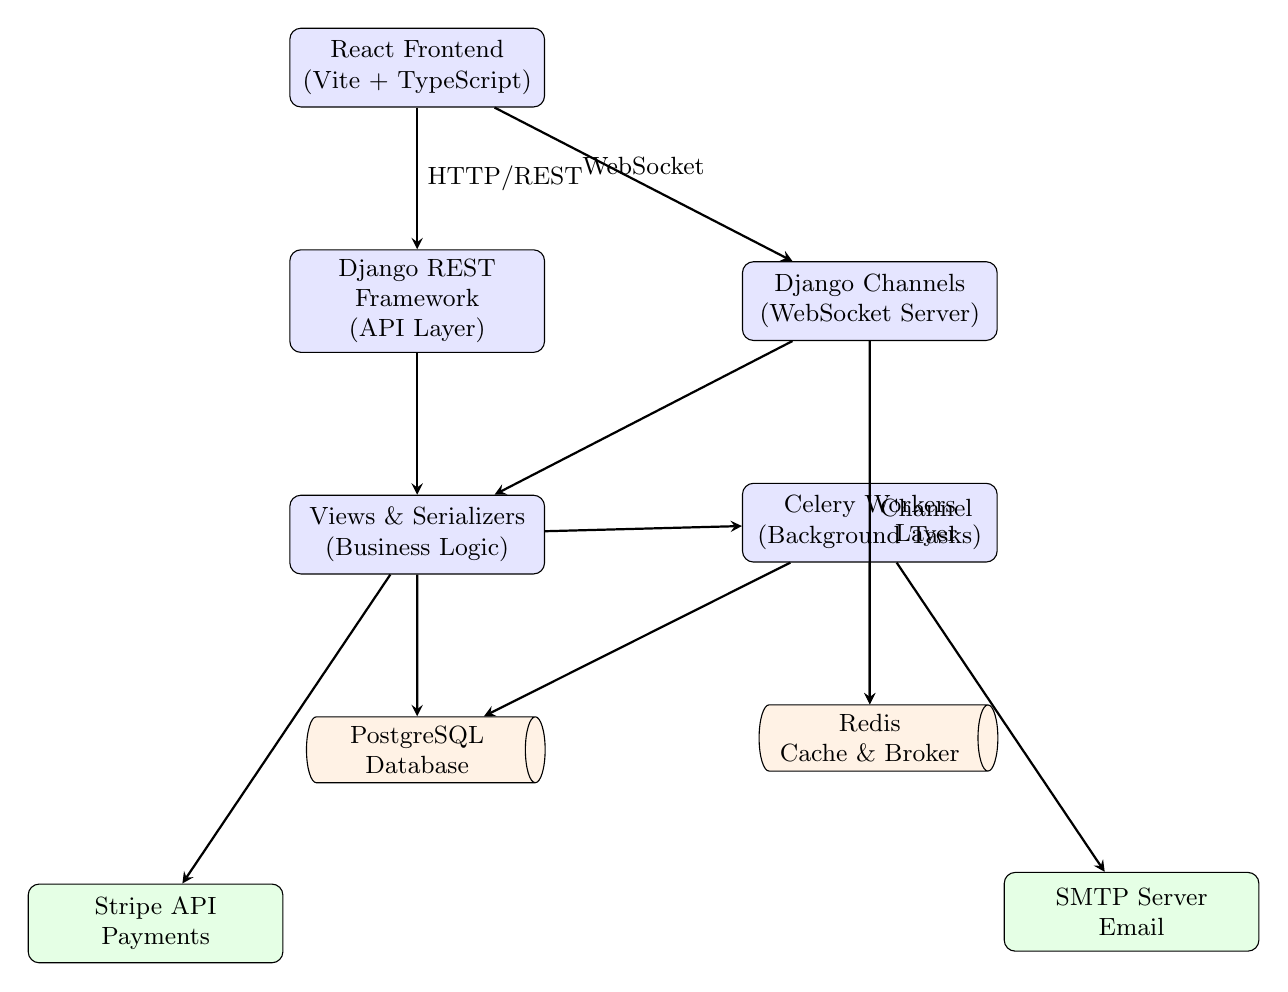
\begin{tikzpicture}[
    node distance=1.8cm,
    every node/.style={font=\small},
    component/.style={rectangle, draw, fill=blue!10, text width=3cm, text centered, rounded corners, minimum height=1cm},
    external/.style={rectangle, draw, fill=green!10, text width=3cm, text centered, rounded corners, minimum height=1cm},
    database/.style={cylinder, draw, fill=orange!10, text width=2.5cm, text centered, minimum height=1cm, aspect=0.3},
    arrow/.style={->, >=stealth, thick}
]

% Frontend Layer
\node[component] (react) {React Frontend\\(Vite + TypeScript)};

% API Gateway
\node[component, below=of react] (drf) {Django REST Framework\\(API Layer)};

% WebSocket Server
\node[component, right=2.5cm of drf] (channels) {Django Channels\\(WebSocket Server)};

% Business Logic Layer
\node[component, below=of drf] (views) {Views \& Serializers\\(Business Logic)};

% Background Tasks
\node[component, below=of channels] (celery) {Celery Workers\\(Background Tasks)};

% Database Layer
\node[database, below=of views] (postgres) {PostgreSQL\\Database};
\node[database, below=of celery] (redis) {Redis\\Cache \& Broker};

% External Services
\node[external, below left=of postgres] (stripe) {Stripe API\\Payments};
\node[external, below right=of redis] (email) {SMTP Server\\Email};

% Arrows
\draw[arrow] (react) -- (drf) node[midway, right] {HTTP/REST};
\draw[arrow] (react) -- (channels) node[midway, above] {WebSocket};
\draw[arrow] (drf) -- (views);
\draw[arrow] (channels) -- (views);
\draw[arrow] (views) -- (postgres);
\draw[arrow] (views) -- (celery);
\draw[arrow] (celery) -- (postgres);
\draw[arrow] (celery) -- (redis);
\draw[arrow] (channels) -- (redis) node[midway, right] {\shortstack{Channel\\Layer}};
\draw[arrow] (views) -- (stripe);
\draw[arrow] (celery) -- (email);

\end{tikzpicture}
\caption{MadeInPK System Architecture}
\end{figure}

\subsection{Database Schema Overview}

The database schema is divided into four logical components, each represented by a separate Entity-Relationship Diagram (ERD):

\subsubsection{ERD 1: User Management \& Authentication}
This ERD covers:
\begin{itemize}
    \item User authentication and profile management
    \item Seller profiles with business information
    \item Location hierarchy (Provinces, Cities, Addresses)
    \item User roles (Buyer, Seller, Both, Admin)
\end{itemize}

\newpage
\begin{center}
\textit{\textbf{[Insert ERD 1 - User Management \& Authentication PDF here]}}
\end{center}
\newpage

\subsubsection{ERD 2: Product Catalog \& Listings}
This ERD covers:
\begin{itemize}
    \item Product base model with categories and images
    \item Auction listings with bidding mechanism
    \item Fixed-price listings with inventory management
    \item Shopping cart and wishlist functionality
    \item Product reviews for fixed-price items
\end{itemize}

\newpage
\begin{center}
\textit{\textbf{[Insert ERD 2 - Product Catalog \& Listings PDF here]}}
\end{center}
\newpage

\subsubsection{ERD 3: Orders \& Payments}
This ERD covers:
\begin{itemize}
    \item Order management for auction and fixed-price purchases
    \item Order items for multi-seller cart orders
    \item Payment processing via Stripe
    \item Seller transfers through Stripe Connect
    \item Feedback system for auction sellers
    \item Payment violations tracking
\end{itemize}

\newpage
\begin{center}
\textit{\textbf{[Insert ERD 3 - Orders \& Payments PDF here]}}
\end{center}
\newpage

\subsubsection{ERD 4: Communication \& Support}
This ERD covers:
\begin{itemize}
    \item Buyer-seller messaging system (Conversations \& Messages)
    \item Notification system for various events
    \item Complaint management system
    \item Email notification tracking
\end{itemize}

\newpage
\begin{center}
\textit{\textbf{[Insert ERD 4 - Communication \& Support PDF here]}}
\end{center}
\newpage

\subsection{System Requirements}

\subsubsection{Functional Requirements}
\begin{enumerate}[leftmargin=*]
    \item \textbf{User Authentication \& Authorization:} System shall support user registration, login, and role-based access control (Buyer, Seller, Admin, Both)
    
    \item \textbf{Dual Listing Types:} System shall allow sellers to create both auction listings (with start/end times) and fixed-price listings (with inventory quantities)
    
    \item \textbf{Real-Time Auction Bidding:} System shall provide real-time bid updates to all connected users viewing an auction using WebSocket technology
    
    \item \textbf{Multi-Seller Cart Checkout:} System shall allow buyers to add products from multiple sellers to a single cart and complete checkout in one transaction
    
    \item \textbf{Automated Auction Processing:} System shall automatically determine auction winners, create orders, and notify bidders when auctions end
    
    \item \textbf{Payment Processing:} System shall integrate with Stripe to securely process payments and create checkout sessions for orders
    
    \item \textbf{Seller Payout Automation:} System shall automatically transfer funds to sellers' Stripe Connect accounts after successful payments, deducting 2\% platform fee
    
    \item \textbf{Order Management:} System shall track order status (pending payment, paid, shipped) and allow sellers to mark items as shipped
    
    \item \textbf{Province-Based Filtering:} System shall allow buyers to filter products by province to discover regional artisans
    
    \item \textbf{Buyer-Seller Messaging:} System shall provide a messaging interface for direct communication between buyers and sellers about products
    
    \item \textbf{Review \& Feedback System:} System shall allow buyers to leave product reviews for fixed-price items and seller feedback for auction purchases
    
    \item \textbf{Notification System:} System shall send in-app and email notifications for bids, auction wins, payments, shipments, and messages
    
    \item \textbf{Wishlist Management:} System shall allow authenticated users to save products to a wishlist for future reference
    
    \item \textbf{Admin Dashboard:} System shall provide administrators with analytics including revenue, orders, users, and seller transfer statistics
    
    \item \textbf{Seller Verification:} System shall allow administrators to verify seller accounts and display verification badges
\end{enumerate}

\subsubsection{Non-Functional Requirements}
\begin{enumerate}[leftmargin=*]
    \item \textbf{Performance:} System shall handle at least 100 concurrent WebSocket connections for real-time auction bidding without degradation
    
    \item \textbf{Scalability:} Database schema shall support horizontal scaling through proper indexing and query optimization
    
    \item \textbf{Security:} System shall use token-based authentication, HTTPS for all communications, and PCI-DSS compliant payment processing via Stripe
    
    \item \textbf{Reliability:} Background tasks (Celery) shall retry failed operations and maintain data consistency across all database transactions
    
    \item \textbf{Availability:} System shall implement proper error handling and logging to maintain 99\% uptime during normal operations
    
    \item \textbf{Data Integrity:} Database shall enforce referential integrity using foreign key constraints and use transactions for multi-step operations
    
    \item \textbf{Usability:} Frontend shall provide responsive design supporting desktop, tablet, and mobile devices with intuitive navigation
    
    \item \textbf{Maintainability:} Codebase shall follow Django best practices with clear separation of concerns (models, views, serializers)
    
    \item \textbf{Real-Time Responsiveness:} WebSocket messages shall be delivered within 100ms for auction bid updates
    
    \item \textbf{Payment Security:} System shall never store credit card information, delegating all payment data to Stripe's secure infrastructure
    
    \item \textbf{Email Delivery:} Notification emails shall be queued and delivered within 5 minutes of triggering events
    
    \item \textbf{API Response Time:} RESTful API endpoints shall respond within 200ms for 95\% of requests under normal load
\end{enumerate}

\newpage

% 3. DISTINGUISHING FEATURES
\section{Distinguishing Features of the Project}

\subsection{Dual Selling Model: Auctions + Fixed-Price}
Unlike traditional e-commerce platforms that only support fixed pricing, MadeInPK offers both:
\begin{itemize}
    \item \textbf{Auction Listings:} Sellers can list unique items with starting prices, allowing competitive bidding to determine final value
    \item \textbf{Fixed-Price Listings:} Standard e-commerce with inventory management, discounts, and multi-quantity purchases
\end{itemize}

This dual model enables sellers to maximize profits on unique handcrafted items through auctions while maintaining steady sales through fixed-price listings.

\subsection{Real-Time Auction Bidding with WebSockets}
\textbf{Implementation Details:}
\begin{itemize}
    \item Django Channels with Redis backend for WebSocket connections
    \item Bidders receive instant updates when they're outbid
    \item Live price updates broadcast to all viewers
    \item Automatic auction ending with winner notification
\end{itemize}

\textbf{Key Benefits:}
\begin{itemize}
    \item Engaging user experience similar to live auctions
    \item Eliminates need for page refreshes
    \item Ensures all bidders have current information
\end{itemize}

\subsection{Multi-Seller Cart Checkout}
\textbf{How it works:}
\begin{itemize}
    \item Buyers can add products from multiple sellers to a single cart
    \item Single checkout process creates one order with multiple \texttt{OrderItem} entries
    \item Platform collects full payment via Stripe Checkout
    \item Automated transfers distribute 98\% of each seller's portion to their Stripe account
    \item Each seller can independently mark their items as shipped
\end{itemize}

This feature mimics large marketplace platforms like Amazon while maintaining transparency in seller payouts.

\subsection{Stripe Connect for Automated Seller Payouts}
\textbf{Financial Flow:}
\begin{enumerate}
    \item Sellers create Stripe Express accounts during onboarding
    \item All payments flow to platform's Stripe account
    \item Platform deducts 2\% commission
    \item Remaining amount automatically transfers to seller's Stripe account
    \item \texttt{SellerTransfer} model tracks all transactions
\end{enumerate}

\textbf{Security \& Compliance:}
\begin{itemize}
    \item Sellers never handle sensitive payment data
    \item Platform complies with PCI-DSS through Stripe
    \item Transparent fee structure (2\% platform fee)
\end{itemize}

\subsection{Province-Based Product Discovery}
\textbf{Implementation:}
\begin{itemize}
    \item Normalized location hierarchy (Province $\rightarrow$ City $\rightarrow$ Address)
    \item Products inherit region from seller's business address or default address
    \item Efficient filtering: \texttt{/api/listings/?province=<id>}
\end{itemize}

\textbf{Business Value:}
\begin{itemize}
    \item Promotes local artisans from specific regions
    \item Buyers can discover products from their province
    \item Supports regional marketing campaigns
\end{itemize}

\subsection{Automated Background Task Processing}
\textbf{Celery Beat Schedule:}
\begin{itemize}
    \item \textbf{Auction Endings} (every 5 minutes): Process ended auctions, create orders, notify winners
    \item \textbf{Payment Deadlines} (every 30 minutes): Block users who fail to pay for won auctions
    \item \textbf{Email Notifications} (every 10 minutes): Send queued notifications via SMTP
\end{itemize}

\textbf{Task Examples:}
\begin{itemize}
    \item Auction winner determination and order creation
    \item Payment deadline enforcement with user blocking
    \item Automated email notifications for various events
    \item Stripe transfer creation after successful payments
\end{itemize}

\subsection{Comprehensive Messaging System}
\textbf{Features:}
\begin{itemize}
    \item Direct buyer-seller conversations about specific products
    \item Message read status tracking
    \item Conversation timestamp updates
    \item Email notifications for new messages
\end{itemize}

\subsection{Dual Review System}
The platform implements two separate review mechanisms:
\begin{itemize}
    \item \textbf{Product Reviews:} For fixed-price products only, linked to verified purchases
    \item \textbf{Seller Feedback:} For auction orders, includes seller rating, communication, shipping speed, and platform rating
\end{itemize}

This separation ensures appropriate feedback mechanisms for different transaction types.

\subsection{Advanced Notification System}
\textbf{Notification Types:}
\begin{itemize}
    \item Bid placed, outbid, auction won/lost
    \item Payment reminders and confirmations
    \item Order status updates (paid, shipped)
    \item Message notifications
    \item Account blocking alerts
\end{itemize}

\textbf{Delivery Channels:}
\begin{itemize}
    \item In-app notifications (stored in database)
    \item Email notifications (queued via Celery)
\end{itemize}

\subsection{Admin Dashboard with Analytics}
\textbf{Key Metrics:}
\begin{itemize}
    \item Total revenue, platform fees, average order value
    \item User statistics (buyers, sellers, blocked users)
    \item Order distribution by status
    \item Top selling products and sellers
    \item Revenue trends (daily, monthly, yearly)
    \item Seller transfer tracking (succeeded, pending, failed)
\end{itemize}

\newpage

% 4. SOURCE CODE SNIPPETS
\section{Source Code Snippets of Main Features}

\subsection{Feature 1: Real-Time WebSocket Auction Bidding}

\subsubsection{WebSocket Consumer Implementation}
The \texttt{AuctionConsumer} class handles real-time bidding using Django Channels:

\begin{lstlisting}[language=Python, caption={WebSocket Consumer for Real-Time Auction (api/consumers.py)}]
class AuctionConsumer(AsyncWebsocketConsumer):
    """WebSocket consumer for real-time auction bidding"""
    
    async def connect(self):
        self.auction_id = self.scope['url_route']['kwargs']['auction_id']
        self.room_group_name = f'auction_{self.auction_id}'
        
        # Join auction group
        await self.channel_layer.group_add(
            self.room_group_name,
            self.channel_name
        )
        
        await self.accept()
        
        # Send current auction status
        auction_data = await self.get_auction_data()
        await self.send(text_data=json.dumps({
            'type': 'auction_status',
            'data': auction_data
        }))
    
    async def receive(self, text_data):
        """Receive bid from WebSocket"""
        data = json.loads(text_data)
        message_type = data.get('type')
        
        if message_type == 'place_bid':
            bid_amount = data.get('amount')
            user = self.scope.get('user')
            
            # Validate and place bid
            result = await self.place_bid(
                self.auction_id, user, bid_amount
            )
            
            if result['success']:
                # Broadcast new bid to all connected users
                await self.channel_layer.group_send(
                    self.room_group_name,
                    {
                        'type': 'new_bid',
                        'bid_data': result['bid_data']
                    }
                )
\end{lstlisting}

\subsubsection{WebSocket URL Routing}
\begin{lstlisting}[language=Python, caption={WebSocket Routing Configuration (api/routing.py)}]
from django.urls import re_path
from . import consumers

websocket_urlpatterns = [
    re_path(
        r'ws/auction/(?P<auction_id>\w+)/$', 
        consumers.AuctionConsumer.as_asgi()
    ),
]
\end{lstlisting}

\subsubsection{Client-Side WebSocket Connection (React)}
\begin{lstlisting}[language=JavaScript, caption={React WebSocket Hook for Auction Bidding}]
const useAuctionWebSocket = (auctionId: string) => {
  const [socket, setSocket] = useState<WebSocket | null>(null);
  const [currentPrice, setCurrentPrice] = useState<number>(0);
  const [bids, setBids] = useState<Bid[]>([]);

  useEffect(() => {
    const ws = new WebSocket(
      `ws://localhost:8000/ws/auction/${auctionId}/`
    );

    ws.onmessage = (event) => {
      const data = JSON.parse(event.data);
      
      if (data.type === 'new_bid') {
        setCurrentPrice(parseFloat(data.data.current_price));
        setBids(prev => [data.data, ...prev]);
      } else if (data.type === 'auction_ended') {
        // Handle auction end
      }
    };

    setSocket(ws);
    return () => ws.close();
  }, [auctionId]);

  const placeBid = (amount: number) => {
    socket?.send(JSON.stringify({
      type: 'place_bid',
      amount: amount
    }));
  };

  return { currentPrice, bids, placeBid };
};
\end{lstlisting}

\subsection{Feature 2: Stripe Connect Integration for Multi-Seller Payouts}

\subsubsection{Creating Stripe Connect Accounts for Sellers}
\begin{lstlisting}[language=Python, caption={Stripe Connect Account Creation (api/stripe\_utils.py)}]
def create_stripe_connect_account(user, return_url, refresh_url):
    """
    Create a Stripe Connect Express account for a seller
    """
    try:
        # Create Connect account for Pakistan (PK)
        account = stripe.Account.create(
            type='express',
            country='PK',
            email=user.email,
            capabilities={
                'transfers': {'requested': True},
            },
            business_type='individual',
            tos_acceptance={
                'service_agreement': 'recipient',
            },
            metadata={
                'user_id': user.id,
                'username': user.username,
            }
        )
        
        # Save account ID to user
        user.stripe_account_id = account.id
        user.save()
        
        # Create account link for onboarding
        account_link = stripe.AccountLink.create(
            account=account.id,
            refresh_url=refresh_url,
            return_url=return_url,
            type='account_onboarding',
        )
        
        return {
            'account_id': account.id,
            'account_link_url': account_link.url,
        }
    except stripe.error.StripeError as e:
        raise Exception(f"Stripe error: {str(e)}")
\end{lstlisting}

\subsubsection{Creating Transfers for Multi-Seller Cart Orders}
\begin{lstlisting}[language=Python, caption={Automated Seller Transfers (api/stripe\_utils.py)}]
def create_transfers_for_cart_order(payment):
    """
    Create transfers to sellers for a multi-seller cart order
    Called after payment is successful
    """
    order = payment.order
    
    if order.order_type != 'cart':
        return
    
    # Group order items by seller
    seller_amounts = OrderItem.objects.filter(
        order=order
    ).values('product__seller').annotate(
        total=Sum('subtotal')
    )
    
    # Get charge ID from payment intent
    payment_intent = stripe.PaymentIntent.retrieve(
        payment.stripe_payment_intent_id
    )
    charge_id = payment_intent.latest_charge
    
    # Create transfer for each seller
    for seller_data in seller_amounts:
        seller_id = seller_data['product__seller']
        subtotal = seller_data['total']
        
        # Calculate platform fee (2%)
        platform_fee = subtotal * Decimal('0.02')
        transfer_amount = subtotal - platform_fee
        
        seller = User.objects.get(id=seller_id)
        
        # Create Stripe transfer
        transfer = stripe.Transfer.create(
            amount=int(transfer_amount * 100),  # Convert to cents
            currency='pkr',
            destination=seller.stripe_account_id,
            source_transaction=charge_id,
            metadata={
                'order_id': order.id,
                'seller_id': seller.id,
                'platform_fee': str(platform_fee),
            }
        )
        
        # Record transfer in database
        SellerTransfer.objects.create(
            payment=payment,
            seller=seller,
            amount=transfer_amount,
            platform_fee=platform_fee,
            stripe_transfer_id=transfer.id,
            status='succeeded',
            completed_at=timezone.now(),
        )
\end{lstlisting}

\subsection{Feature 3: Automated Auction Processing with Celery}

\subsubsection{Celery Task for Processing Ended Auctions}
\begin{lstlisting}[language=Python, caption={Automated Auction Ending Task (api/tasks.py)}]
@shared_task
def check_auction_endings():
    """Check for auctions that have ended and process winners"""
    now = timezone.now()
    ended_auctions = AuctionListing.objects.filter(
        status='active',
        end_time__lte=now
    ).select_related('product', 'product__seller')
    
    for auction in ended_auctions:
        # Get the winning bid
        winning_bid = auction.bids.filter(is_winning=True).first()
        
        if winning_bid:
            # Update auction with winner
            auction.winner = winning_bid.bidder
            auction.status = 'ended'
            auction.save()
            
            # Calculate amounts
            total_amount = winning_bid.amount
            platform_fee = total_amount * Decimal('0.02')
            seller_amount = total_amount - platform_fee
            
            # Create order
            order = Order.objects.create(
                order_number=f"AUC-{uuid.uuid4().hex[:12].upper()}",
                buyer=winning_bid.bidder,
                seller=auction.product.seller,
                product=auction.product,
                order_type='auction',
                auction=auction,
                total_amount=total_amount,
                platform_fee=platform_fee,
                seller_amount=seller_amount,
                shipping_address=winning_bid.bidder.addresses
                    .filter(is_default=True).first(),
                status='pending_payment',
                payment_deadline=now + timedelta(hours=24)
            )
            
            # Create Stripe payment URL
            payment_result = create_payment_intent_for_order(
                order=order,
                success_url=f"http://localhost:8000/api/payments/success/",
                cancel_url=f"http://localhost:5173/auctions/{auction.id}"
            )
            order.payment_url = payment_result['checkout_url']
            order.save()
            
            # Notify winner
            Notification.objects.create(
                user=winning_bid.bidder,
                notification_type='auction_won',
                title='Congratulations! You won the auction',
                message=f'You won {auction.product.name}. '
                        f'Please pay within 24 hours.',
                auction=auction,
                order=order
            )
            
            # Send email notification
            send_auction_won_email.delay(order.id)
\end{lstlisting}

\subsubsection{Celery Beat Schedule Configuration}
\begin{lstlisting}[language=Python, caption={Periodic Task Schedule (MadeInPK/celery.py)}]
app.conf.beat_schedule = {
    'check-auction-endings': {
        'task': 'api.tasks.check_auction_endings',
        'schedule': crontab(minute='*/5'),  # Every 5 minutes
    },
    'check-payment-deadlines': {
        'task': 'api.tasks.check_payment_deadlines',
        'schedule': crontab(minute='*/30'),  # Every 30 minutes
    },
    'send-pending-notifications': {
        'task': 'api.tasks.send_pending_notifications',
        'schedule': crontab(minute='*/10'),  # Every 10 minutes
    },
}
\end{lstlisting}

\newpage

% 5. CONTRIBUTIONS OF MEMBERS
\section{Contributions of Members}

\begin{table}[H]
\centering
\footnotesize
\begin{tabular}{|p{2.2cm}|p{4.5cm}|p{7cm}|}
\hline
\textbf{Member} & \textbf{Responsibilities} & \textbf{Key Contributions \& Technologies} \\
\hline
\textbf{Muhammad Abdullah Khan}

\vspace{0.1cm}
SE-23061 & 
Backend Development, Database Design, API Implementation &
$\bullet$ Designed 24-model normalized database schema

$\bullet$ Implemented Django models and migrations

$\bullet$ Created 50+ REST API endpoints (DRF)

$\bullet$ Developed serializers and validators

$\bullet$ Province-based filtering system

\vspace{0.1cm}
\textit{Tech: Django 5.2.7, PostgreSQL, Python} \\
\hline
\textbf{Haris Masood}

\vspace{0.1cm}
SE-23088 & 
Payment Integration, Background Tasks, Webhooks &
$\bullet$ Integrated Stripe and Stripe Connect

$\bullet$ Automated seller payouts (2\% fee)

$\bullet$ Set up Celery task queue and Beat scheduler

$\bullet$ Created payment webhook handlers

$\bullet$ Developed email notification system

\vspace{0.1cm}
\textit{Tech: Stripe API, Celery, Redis, SMTP} \\
\hline
\textbf{M. Huzaifa Hassan}

\vspace{0.1cm}
SE-23089 & 
Real-Time Features, Frontend Architecture, WebSockets &
$\bullet$ Implemented WebSocket consumers for auctions

$\bullet$ Set up Django Channels with Redis

$\bullet$ Created React app structure with TypeScript

$\bullet$ Developed Context API state management

$\bullet$ Built custom WebSocket hooks

\vspace{0.1cm}
\textit{Tech: Django Channels, React 18, TypeScript, Vite} \\
\hline
\textbf{Muhammad Rafay}

\vspace{0.1cm}
SE-23100 & 
Frontend UI/UX, Dashboard, Component Design &
$\bullet$ Designed and implemented all UI pages

$\bullet$ Created responsive product catalog

$\bullet$ Built multi-seller cart and checkout

$\bullet$ Developed admin analytics dashboard

$\bullet$ Implemented messaging and notifications UI

\vspace{0.1cm}
\textit{Tech: React, Tailwind CSS, shadcn/ui, Recharts} \\
\hline
\end{tabular}
\caption{Team Member Contributions Summary}
\end{table}

\subsection{Collaborative Efforts}
The team worked collaboratively on:
\begin{itemize}
    \item Joint database schema design and normalization sessions
    \item API endpoint design and documentation
    \item Code reviews and pair programming for complex features
    \item Integration testing between frontend and backend
    \item Deployment configuration and environment setup
    \item Git version control and GitHub collaboration
\end{itemize}

\newpage

% 6. FUTURE EXPANSIONS
\section{Future Expansions}

\subsection{AI-Powered Recommendation System}
Implement machine learning algorithms for personalized product recommendations:
\begin{itemize}
    \item \textbf{Collaborative Filtering:} Suggest products based on similar user purchase patterns
    \item \textbf{Content-Based Filtering:} Recommend items similar to viewed/wishlisted products
    \item \textbf{NLP Search:} Enable conversational product queries using natural language
    \item \textbf{AI Chatbot:} Automated customer support for FAQs and purchase guidance
    \item \textbf{Impact:} Increased user engagement and conversion rates through personalization
\end{itemize}

\subsection{Mobile Application Development}
Cross-platform mobile app (React Native/Flutter) with native features:
\begin{itemize}
    \item \textbf{Push Notifications:} Real-time alerts for bids, outbid warnings, orders, messages
    \item \textbf{Mobile Payment Integration:} Support for JazzCash and Easypaisa
    \item \textbf{Biometric Authentication:} Fingerprint/face recognition for secure login
    \item \textbf{Camera Integration:} Direct photo uploads for sellers
    \item \textbf{Offline Mode:} Browse cached products without internet
    \item \textbf{Touch-Optimized Bidding:} Gesture-based auction interface
\end{itemize}

\subsection{Advanced Analytics Dashboard}
Business intelligence tools for data-driven decisions:
\begin{itemize}
    \item \textbf{Sales Forecasting:} ML models for revenue and demand prediction
    \item \textbf{Customer Segmentation:} Identify high-value buyers and behaviors
    \item \textbf{Seller Metrics:} Conversion rates, view-to-purchase ratios, pricing insights
    \item \textbf{Automated Reports:} Daily/weekly/monthly KPI summaries
    \item \textbf{Interactive Visualizations:} Charts, graphs, and heatmaps (D3.js/Recharts)
    \item \textbf{Market Trends:} Category popularity, peak times, regional preferences
\end{itemize}

\subsection{Logistics \& Shipping Integration}
Streamlined fulfillment with local courier services:
\begin{itemize}
    \item \textbf{Courier Integration:} TCS, Leopards Courier, M\&P Express APIs
    \item \textbf{Auto-Generated Labels:} Shipping labels with tracking numbers
    \item \textbf{Real-Time Tracking:} Status updates for buyers and sellers
    \item \textbf{Cost Calculator:} Compare quotes from multiple couriers
    \item \textbf{Warehouse Management:} Multi-location inventory, low-stock alerts, barcode scanning
    \item \textbf{Smart Routing:} Optimized delivery routes for sellers
    \item \textbf{Flexible Delivery:} Scheduled slots, alternate drop-offs, express shipping
\end{itemize}

\newpage

% CONCLUSION
\section{Conclusion}

MadeInPK represents a comprehensive e-commerce solution specifically designed to empower Pakistani artisans and manufacturers through a dual selling model combining traditional fixed-price sales with competitive auction mechanisms. The platform successfully integrates modern web technologies including Django REST Framework, React with TypeScript, WebSockets for real-time communication, and Stripe Connect for automated payment processing.

\subsection{Key Achievements}
\begin{itemize}
    \item \textbf{Robust Database Design:} Implemented a normalized database schema with 20+ models covering users, products, orders, payments, and communication
    \item \textbf{Real-Time Features:} Developed live auction bidding using WebSocket technology with instant price updates
    \item \textbf{Automated Processing:} Integrated Celery for background tasks including auction endings, payment reminders, and email notifications
    \item \textbf{Secure Payments:} Implemented Stripe Connect for seamless seller onboarding and automated payouts with 2\% platform fee
    \item \textbf{Multi-Seller Support:} Created a sophisticated cart system supporting purchases from multiple sellers in a single transaction
    \item \textbf{Regional Discovery:} Enabled province-based filtering to promote local artisans
\end{itemize}

\subsection{Learning Outcomes}
Through this project, the team gained extensive experience in:
\begin{itemize}
    \item Full-stack web development with modern frameworks
    \item Database design and optimization for complex e-commerce systems
    \item Real-time communication using WebSocket technology
    \item Payment gateway integration and financial transaction handling
    \item Background task processing and job scheduling
    \item RESTful API design and implementation
    \item State management in large React applications
\end{itemize}

\subsection{Impact}
MadeInPK provides a scalable foundation for:
\begin{itemize}
    \item Supporting local businesses and artisans
    \item Creating transparent marketplace dynamics
    \item Facilitating fair price discovery through auctions
    \item Ensuring secure and automated financial transactions
    \item Building trust through comprehensive review systems
\end{itemize}

The platform is production-ready and can be deployed to serve real users, with clear paths for future enhancements as outlined in Section 6.

\vspace{1cm}

\hrule

\vspace{0.5cm}

\begin{center}
\textit{This project demonstrates the practical application of e-commerce concepts and modern web technologies in building a scalable marketplace platform that addresses real-world business needs of Pakistani artisans and manufacturers.}
\end{center}

\newpage

% APPENDICES
\appendix

\section{Database Statistics}

\subsection{Model Count}
\begin{table}[H]
\centering
\begin{tabular}{|l|c|}
\hline
\textbf{Category} & \textbf{Number of Models} \\
\hline
User Management & 4 (User, SellerProfile, Province, City, Address) \\
Products & 5 (Product, ProductImage, Category, AuctionListing, FixedPriceListing) \\
Orders & 6 (Order, OrderItem, Payment, SellerTransfer, Feedback, PaymentViolation) \\
Shopping & 4 (Cart, CartItem, Wishlist, ProductReview) \\
Communication & 4 (Conversation, Message, Notification, Complaint) \\
Auctions & 1 (Bid) \\
\hline
\textbf{Total} & \textbf{24 Models} \\
\hline
\end{tabular}
\caption{Database Models Summary}
\end{table}

\subsection{API Endpoints Count}
\begin{table}[H]
\centering
\begin{tabular}{|l|c|}
\hline
\textbf{Category} & \textbf{Number of Endpoints} \\
\hline
Authentication & 4 (register, login, logout, profile) \\
Products & 6 (CRUD + image management) \\
Auctions & 5 (CRUD + bidding) \\
Fixed-Price Listings & 6 (CRUD + purchase + toggle status) \\
Orders & 4 (list, detail, mark shipped) \\
Cart & 5 (view, add, update, remove, checkout) \\
Wishlist & 4 (CRUD operations) \\
Reviews & 4 (CRUD for product reviews) \\
Feedback & 4 (CRUD for seller feedback) \\
Messaging & 3 (conversations, messages, send) \\
Notifications & 3 (list, mark read, mark all read) \\
Stripe Connect & 3 (create account, status, refresh) \\
Admin & 3 (statistics, earnings, transactions) \\
\hline
\textbf{Total} & \textbf{50+ Endpoints} \\
\hline
\end{tabular}
\caption{RESTful API Endpoints Summary}
\end{table}

\section{Technology Versions}

\begin{table}[H]
\centering
\begin{tabular}{|l|l|}
\hline
\textbf{Technology} & \textbf{Version} \\
\hline
Django & 5.2.7 \\
Django REST Framework & Latest \\
PostgreSQL & 15-alpine \\
Redis & 7-alpine \\
Python & 3.10+ \\
React & 18 \\
TypeScript & Latest \\
Vite & Latest \\
Node.js & 18+ \\
Celery & Latest \\
Django Channels & Latest \\
Stripe API & Latest \\
\hline
\end{tabular}
\caption{Technology Stack Versions}
\end{table}

\section{References}

\begin{enumerate}
    \item Django Documentation: \url{https://docs.djangoproject.com/}
    \item Django REST Framework: \url{https://www.django-rest-framework.org/}
    \item Django Channels: \url{https://channels.readthedocs.io/}
    \item Celery Documentation: \url{https://docs.celeryproject.org/}
    \item Stripe API Documentation: \url{https://stripe.com/docs/api}
    \item Stripe Connect Guide: \url{https://stripe.com/docs/connect}
    \item React Documentation: \url{https://react.dev/}
    \item TypeScript Handbook: \url{https://www.typescriptlang.org/docs/}
    \item WebSocket Protocol: \url{https://datatracker.ietf.org/doc/html/rfc6455}
    \item PostgreSQL Documentation: \url{https://www.postgresql.org/docs/}
\end{enumerate}

\end{document}
